\documentclass[conference]{IEEEtran}
%%
\def\BibTeX{{\rm B\kern-.05em{\sc i\kern-.025em b}\kern-.08em
    T\kern-.1667em\lower.7ex\hbox{E}\kern-.125emX}}
%%
\usepackage{cite}
\usepackage{amsmath,amssymb,amsfonts}
\usepackage{url}
\usepackage{algorithmic}
\usepackage{graphicx}
\usepackage{textcomp}
\usepackage{xcolor}
\usepackage{lettrine}
\usepackage{listings}
\usepackage{booktabs}
\usepackage{hyperref}
\usepackage{pdfpages}

%% Reusable screenshot placeholder box (compiles without image files)
\newcommand{\screenshotbox}[2]{%
  \fbox{\parbox[c][#2][c]{0.95\linewidth}{\centering\textbf{Screenshot Placeholder}\\[0.4em]#1}}
}

%% Code listing style
\lstset{
  basicstyle=\ttfamily\small,
  breaklines=true,
  frame=single,
  backgroundcolor=\color{gray!10},
  keywordstyle=\color{blue},
  commentstyle=\color{green!60!black},
  stringstyle=\color{orange!80!black}
}

\begin{document}

%%% Uncomment the line below after obtaining your NCI Project Cover Sheet from Moodle
% \includepdf{nci-project-cover-sheet.pdf}

\title{SentriVault: A Cloud-Native Secure Secrets and Access Governance Platform}

\author{Ishan\\
StudentId: x25175661\\
Cloud DevSecOps, MSc in Cloud Computing\\
National College of Ireland Dublin, IRELAND\\
Email: x25175661@student.ncirl.ie\\
URL: \url{www.ncirl.ie}\\
Deployed Application URL: \url{[Your-Deployment-URL]}\\
GitHub Repository: \url{https://github.com/[your-repo]/DevOpSec}}

\maketitle

\begin{abstract}
In the present times web-apps, cloud service users, SaaS Providers, or any software service provider / holder has an obligation to store variety of confidential secrets e.g., API Keys, Database passwords, SSL certs, Access tokens, Auth secret etc. The exposure of these secrets hold a risk of companies facing major financial and reputational hit. The report introduces SentriVault -- a cloud-native secrets management and governance platform which is build using React, Node.js/Express and PostgreSQL. The platform's primary purpose is to provide org's security admins a dashboard and safe vault to store and manage all of the critical secrets and environment configurables, further leveraging the access control over them for the employees and RBAC - (role based access control) system and an immutable audit log system to log every change being made on the platform to ensure accountibility and tracibility. Furthermore, the platform provides the leverage to encrypt and decrypt secrets using variety of algorithms on the platform itself. The platform has been deployed on AWS Elastic Beanstalk (backend) and Amazon S3 Hosting service (Frontend). For static analysis, the platform is using TypeScript strict mode, ESLint and npm audit along with SonarQube. Upon performing the functional testing, during the development phases, several security and usability bugs have been caught and fixed such as - decryption payload error , revoke access control error etc. The results demonstrate how a simple open source cloud based platform can provide a secure and strong secret storage and governance service.
\end{abstract}

\begin{IEEEkeywords}
secrets management, RBAC, AES-256-GCM, static code analysis, DevSecOps, CI/CD, audit logging
\end{IEEEkeywords}

%% ─────────────────────────────────────────────
\section{Introduction}
\label{sec:intro}

\lettrine[findent=2pt]{\fbox{\textbf{M}}}{ }odern cloud systems usually hold various secrets such as API Keys, passwords, SSH Keys, certificates. Projects having microservices usually have continuously growing secret count. Having even a single secret leak can lead to a major breach. Recent surveys have shown that credential leaks are among the most common attack paths. SentriVault is designed to demonstrate how a secure secret platform with open source tools and negligible cost AWS services can be a solution to ensure various security goals:

\begin{itemize}
    \item \textbf {Confidentiality} - Secret values are being encrypted before storage with symmetric authenticated encryption along with automatic secret roation period.
    \item \textbf {Least-Privilege Access} - Every API routes are designed to be gated by a unique RBAC permission key which is evaluated at the runtime, even passing a valid token via XSS with lacking RBAC permission would return HTTP 403.
    \item \textbf {Accountability} - Each and every access event is logged in the audit log system with immutability covering actor , target, action, success state, source IP etc.
    \item \textbf {Security Summary} - The platform provides active summary report for currently stored secrets and suggestions to improve security and mitigate risk divided into low medium and high severity.
\end{itemize}


This report demonstrated the design, implementation, testing and deployment of the platform - SentriVault. The project uses React + TypeScript for frontend , Express + Node.js for backend, PostgreSQL for database and GitHub Actions for CI/CD pipeline.


%% ─────────────────────────────────────────────
\section{Project Requirements}
\label{sec:requirements}

\lettrine[findent=2pt]{\fbox{\textbf{T}}}{ }his section explains the current project stack and working of each layer in SentriVault.

\subsection{Required Project Stack}

The implementation includes the following stack:

\begin{itemize}
  \item Frontend: React js, TypeScript 5, React Router
  \item Backend: Node.js 20, Express 5, TypeScript 5, Zod validation
  \item Database: PostgreSQL 16 with role-based schema and audit tables
  \item Security: JWT authentication, bcrypt password hashing, RBAC middleware, secret encryption algorithms
  \item DevOps: GitHub Actions for CI/CD, AWS Elastic Beanstalk for backend deployment, Amazon S3 for frontend deployment
  \item Quality and security checks: TypeScript strict mode, ESLint, npm audit and SonarQube
\end{itemize}

\subsection{How the Stack Works Together}

The user accesses the React web app via public url and creates an account or sign in to an existing account. The app sends request to our active express backend on BeanStalk. Backend validates the request with JWT and RBAC permissions, then validated the body with Zod. Upon the validation passes, the backend writes the data in PostgreSQL. Backend encryptes secrets before writing it to the database, and decrypts only when requested via platform's valid route. Every action is written in the audit log table. In production, GitHub Actions helps in building both frontend and backend and deploys to AWS services.


\subsection{Encryption Algorithm Used in SentriVault}

Before data is written to PostgreSQL, SentriVault uses AES-256-GCM (Advanced Encryption Standard, 256-bit key, Galois/Counter Mode) to protect secret values. This option gives you both privacy and security in one step:
The authentication tag stops tampering that goes undetected, while the ciphertext protects the secret content. The backend makes a new random IV (nonce) for each encryption operation.
When decrypting, the service first checks the authentication tag and only sends back plaintext if the integrity checks pass.
The encrypted payload that the app keeps includes the ciphertext and the cryptographic metadata needed to decrypt it safely.

\begin{table}[h]
\centering
\caption{Encryption specification used in SentriVault\label{table:encryption-spec}}
\renewcommand{\arraystretch}{1.08}
\begin{tabular}{||l l||}
\hline
\textbf{Parameter} & \textbf{Value in Application} \\
\hline\hline
Cipher algorithm & AES-256-GCM \\
Key length & 256 bits (32 bytes) \\
IV (nonce) length & 96 bits (12 bytes) \\
Authentication tag length & 128 bits (16 bytes) \\
Stored encrypted fields & \texttt{value}, \texttt{iv}, \texttt{auth\_tag}, \texttt{algorithm} \\
Security property & Confidentiality + integrity \\
\hline
\end{tabular}
\end{table}

Table II lists some of the most common classical and modern methods that are often talked about in security classes. SentriVault only uses AES-256-GCM to protect production secrets because old methods aren't safe against new attacks.

\begin{table}[h]
\centering
\caption{Encryption/encoding methods considered\label{table:method-comparison}}
\renewcommand{\arraystretch}{1.06}
\begin{tabular}{||l l l||}
\hline
\textbf{Method} & \textbf{Category}  \\
\hline\hline
Caesar cipher & Classical substitution cipher  \\
Vigenere cipher & Classical polyalphabetic cipher \\
Morse code & Encoding (not encryption) \\
Base64 & Encoding (not encryption) \\
AES-256-GCM & Modern authenticated symmetric encryption  \\
\hline
\end{tabular}
\end{table}

\subsection{Project Code Directory Evidence}

\begin{figure}[ht]
    \centering
    \includegraphics[width=8.0cm]{Screenshot 2026-04-01 at 18.15.49.png}
    \caption{Project code directory screenshot placeholder.}
    \label{fig:project-directory-shot}
\end{figure}


%% ─────────────────────────────────────────────
\section{Continuous Integration, Continuous Delivery and Deployment}
\label{sec:cicd}

\lettrine[findent=2pt]{\fbox{\textbf{T}}}{ }his section demonstrates the CI/CD pipeline and it's architecture, workflow of new commit and changes and        the employed tools during the process.

\subsection{Architecture Overview}

SentriVault is fundamentally a three-tier application -- React 18 single-page application (SPA) communicating over HTTP with a REST API build in Node.js and Express, which writes to PostgreSQL. Figure 2. illustrated the deployment structure.

\begin{figure}[ht]
\begin{center}
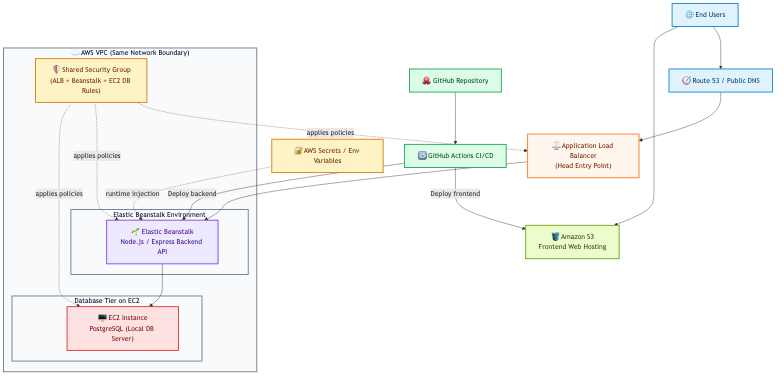
\includegraphics[width=\linewidth]{deployment-architecture.png}
\caption{Three Tier Architecture\label{fig:arch}}
\end{center}
\end{figure}

%% ─────────────────────────────────────────────

In production, the frontend is accessible via a static Vite bundle from AWS S3 and backend runs in AWS Beanstalk working behind an Application Load Balancer under the same VPC. Table I lists all the core dependencies.

\begin{table}[h]
\centering
\caption{Technology Stack\label{table:stack}}
\renewcommand{\arraystretch}{1.05}
\begin{tabular}{||l l||}
\hline
\textbf{Component} & \textbf{Technology} \\[0.5ex]
\hline\hline
Frontend Framework & React 18 + TypeScript 5 \\
Build Tool & Vite 5 \\
Routing & React Router v6 \\
API Framework & Express 5 \\
Backend Language & Node.js 20 + TypeScript 5 \\
Request Validation & Zod 3 \\
Database & PostgreSQL 16 \\
Authentication & JSON Web Tokens (JWT) \\
Password Hashing & bcrypt (cost 12) \\
Database Driver & node-postgres (pg) \\
CI/CD Orchestration & GitHub Actions \\
Infrastructure & AWS (Elastic Beanstalk, S3 Web Hosting, EC2) \\
\hline
\end{tabular}
\end{table}

\subsection{CI/CD Pipeline Design}

The workflow (stored in \texttt{.github/workflows/ci-cd.yml}) implements a three stage pipeline -- Continuous Integeration (build and test), Continuous Delivery (backend to Elastic Beanstalk) and Continuous Delivery (frontend to S3)

\begin{figure}[ht]
\begin{center}
\includegraphics[width=\linewidth]{cd.png}
\caption{Pipeline-CD Overview\label{fig:arch}}
\end{center}
\end{figure}

\begin{figure}[ht]
\begin{center}
\includegraphics[width=\linewidth]{ci-cd.png}
\includegraphics[width=\linewidth]{CI-CD2.png}
\caption{Continuous Integeration + Continuous Development (Backend + Frontend )\label{fig:arch}}
\end{center}
\end{figure}

\subsubsection{Continuous Integration}

On each push to the \texttt{main} branch, the CI job:

\begin{enumerate}
  \item Checks out the repository
  \item Sets up Node.js 20
  \item Installs backend dependencies through \texttt{npm ci}
  \item Compiles backend TypeScript with \texttt{npm run build}
  \item Installs frontend dependencies through \texttt{npm ci}
  \item Compiles frontend TypeScript through \texttt{npm run build}
\end{enumerate}

If any one of the steps fails, the job fails and no deployment happens. TypeScript \texttt{strict: true} mode works as an enforced static type check - any type or space error fails/stops the build. This constraint prevents type errors/bugs from deploying to production.

\subsubsection{Continuous Deployment — Backend}

On successful CI completion, the CD Backend job:

\begin{enumerate}
  \item Zips the built backend application (excluding \texttt{node\_modules/})
  \item Generates a versioned deploy label: \texttt{devopsec-backend-\$\{git\ sha\}-r\$\{run\_id\}}
  \item Uploads the ZIP to an already configured S3 bucket
  \item Instantiate the AWS Elastic Beanstalk API to deploy the new version of backed build.
\end{enumerate}

The backend deployment uses various environment variables implemented from GitHub Actions secrets at runtime: \texttt{ENCRYPTION\_KEY}, \texttt{DATABASE\_URL}, \texttt{JWT\_SECRET}, \texttt{AWS\_ACCESS\_KEY\_ID}, \texttt{AWS\_SECRET\_ACCESS\_KEY}. These credentials never appear in repository files due to security principles.

\subsubsection{Continuous Deployment — Frontend}

The CD Frontend job:

\begin{enumerate}
  \item Builds the Vite production bundle via \texttt{npm run build}
  \item Syncs up the \texttt{dist/} directory to S3 using \texttt{aws s3 sync}
\end{enumerate}

 The deployed frontend is served from \texttt{https://devopsec.example.com}. All API requests go to the backend at \texttt{}.

\subsection{Deployment Function — Code Change Flow}

Any changed being made follows the following workflow:

\begin{enumerate}
  \item Modifies source files (e.g., \texttt{backend/src/modules/secrets/routes.ts})
  \item Commits and pushes the branch to GitHub: \texttt{git push origin feature/my-change}
  \item Opens a pull request against \texttt{main}
  \item The CI workflow triggers automatically on the pull request, building both backend and frontend
  \item Upon approval and merge, the code merges to \texttt{main}
  \item The CI workflow runs again on \texttt{main}; on success, the CD jobs deploy the builds to Elastic Beanstalk and S3
\end{enumerate}

\begin{figure}[ht]
\begin{center}
\includegraphics[width=\linewidth]{cc.png}
\caption{Code-change PR to initiate CI-CD.\label{fig:pipeline-run}}
\end{center}
\end{figure}

\begin{figure}[ht]
\begin{center}
\includegraphics[width=\linewidth]{CI-CD2.png}
\caption{Pipeline run-in-action screenshot placeholder.\label{fig:pipeline-run}}
\end{center}
\end{figure}

\subsubsection{Production Result Evidence}

To clearly show production success in Fig 7.

\begin{figure}[ht]
\begin{center}
\includegraphics[width=\linewidth]{app1.png}
\includegraphics[width=\linewidth]{app2.png}
\caption{Production Application.\label{fig:pipeline-run}}
\end{center}
\end{figure}

\begin{figure}[ht]
\begin{center}
\includegraphics[width=\linewidth]{aws.png}
\caption{Production backend status.\label{fig:pipeline-run}}
\end{center}
\end{figure}

\subsection{Database and Local Development}

Local development begins with:

\begin{lstlisting}[language=bash]
cd backend && npm install && npm run build && npm run dev
cd frontend && npm install && npm run dev
\end{lstlisting}

This connects to the already configured PostgreSQL server on EC2 on \texttt{Elastic IP / Private IP:5432}, the Express server on \texttt{localhost:4000}, and the Vite dev server on \texttt{localhost:5173}. The frontend's \texttt{.env.local} sets \texttt{http://beanstalkURL:4000/api/v1}.

All database schema migration is being handled via backend/prisma-or-sql/ and applied via deployment script (ci-cd.yml) to the EC2 PostgreSQL server.

%% ─────────────────────────────────────────────
\section{Static Code Analysis and Security Vulnerability Analysis}
\label{sec:sca}

\lettrine[findent=2pt]{\fbox{\textbf{T}}}{ }his section demonstrates the tools used, key findings and fixes.

\subsection{Tools Used}

The project used three core checks during CI and local verification:

\begin{itemize}
  \item \textbf{TypeScript strict mode} to catch type-strict issues before deployment.
  \item \textbf{ESLint} to detect unsafe code patterns and code-quality issues.
  \item \textbf{npm audit} to detect known dependency vulnerabilities.
\end{itemize}

\begin{figure}[ht]
\begin{center}
\includegraphics[width=\linewidth]{SQ.png}
\caption{SonarQube Result.\label{fig:pipeline-run}}
\end{center}
\end{figure}

\subsection{Key Findings and Fixes (Summary)}

\begin{table}[h]
\centering
\caption{Static analysis and security fixes summary\label{table:vulns}}
\renewcommand{\arraystretch}{1.1}
\begin{tabular}{||p{1.1cm} p{2.0cm} p{2.8cm}||}
\hline
\textbf{Type} & \textbf{Finding} & \textbf{Fix} \\[0.5ex]
\hline\hline
Crypto & Invalid handling in decrypt path & Added auth-tag validation before decryption of cypher \\
\hline
Crypto & Incomplete cipher copy payload & Copied to clipboard full JSON payload: value, iv, auth\_tag, algorithm \\
\hline
Access & Revoked secrets still listed & Added additional query filter \\
\hline
Runtime & Clipboard API failed in non-HTTPS & Added fallback copy method \\
\hline
Type safety & Missing audit action type & Added \texttt{update\_secret} to \texttt{AuditAction}\\
\hline
\end{tabular}
\end{table}

\subsection{Result Snapshot}

Final Check showed one type issue fixed an no high-priority ESLint errors.

\begin{figure}[ht]
\begin{center}
\includegraphics[width=\linewidth]{fix.png}
\caption{Static analysis output.\label{fig:static-summary-shot}}
\end{center}
\end{figure}

%% ─────────────────────────────────────────────
\section{Conclusions}
\label{sec:conclusions}

\lettrine[findent=2pt]{\fbox{\textbf{T}}}{ }his project proves that we can build a secure secrets platform with open source tools and near to free tier AWS services available to provide secure storage and access governance system.
\subsection{Key Findings}

\begin{enumerate}
  \item \textbf{Static analysis catches real defects:} Typescript strict mode caught missing audit action value and a bug that dynamic testing might have missed.
  \item \textbf{Defence-in-depth is practical:} Layered architecture of encryption, RBAC , auditing altogether provides a solid solution in the form of a PAAS (platform as a service)
  \item \textbf{RBAC runtime enforcement scales:} Live database permission checks (rather than JWT claims) immediatly revokes the token rather than rotating it altogether.
\end{enumerate}

\subsection{Reflection and Lessons Learned}

If this project is implemented again, these improvements should be done first:

\begin{itemize}
  \item \textbf{Key management:} To use an AWS KMS or HashiCorp Vault for hardware-backed key storage service rather than environment variables.
  \item \textbf{PBKDF2 key derivation:} Replace SHA-256 hashing with PBKDF2 or \texttt{scrypt} and a salt to harden against brute-force attacks which are getting more common in the modern times.
  \item \textbf{Rate limiting:} Implement rate limiting on authentication endpoints to prevent credential-stuffing attacks.
  \item \textbf{Refresh token rotation:} Complete implementation of JWT refresh-token rotation so that any compromised tokens have a limited -fixed lifetime.
  \item \textbf{Runtime secrets monitoring:} A live notification service which can alert admin and designated employee users regarding any active high risk or severity caught by the platform-analyzer.
\end{itemize}


In short, SentriVault is a good way to manage secrets on a large scale with security controls that can be verified. Adding static analysis to the deployment pipeline, along with access control and immutable auditing at runtime, makes the system much stronger than traditional ad-hoc secret storage methods.


%% ─────────────────────────────────────────────

\begin{thebibliography}{99}


\bibitem{verizon2023}
Verizon, "2023 Data Breach Investigations Report," 2023. [Online]. Available: https://www.verizon.com/business/resources/reports/dbir/. [Accessed: Apr. 1, 2026].

\bibitem{owasp2021}
OWASP Foundation, "OWASP Top 10: The Ten Most Critical Web Application Security Risks," 2021. [Online]. Available: https://owasp.org/www-project-top-ten/. [Accessed: Apr. 1, 2026].

\bibitem{ibm2024}
IBM Security, "Cost of a Data Breach Report 2024," 2024. [Online]. Available: https://www.ibm.com/reports/data-breach. [Accessed: Apr. 1, 2026].

\bibitem{enisa2023}
European Union Agency for Cybersecurity (ENISA), "ENISA Threat Landscape 2023," 2023. [Online]. Available: https://www.enisa.europa.eu/publications/enisa-threat-landscape-2023. [Accessed: Apr. 1, 2026].

\bibitem{nist-csf20}
National Institute of Standards and Technology (NIST), "The NIST Cybersecurity Framework (CSF) 2.0," NIST CSWP 29, 2024.

\bibitem{nist-80053r5}
National Institute of Standards and Technology (NIST), "Security and Privacy Controls for Information Systems and Organizations," NIST SP 800-53 Rev. 5, 2020 (upd. 2023).

\bibitem{ferraiolo-kuhn-1992}
D. F. Ferraiolo and D. R. Kuhn, "Role-Based Access Controls," in \textit{Proc. 15th NIST-NCSC National Computer Security Conference}, Baltimore, MD, USA, 1992, pp. 554--563.

\bibitem{sandhu-rbac-1996}
R. Sandhu, E. J. Coyne, H. L. Feinstein, and C. E. Youman, "Role-Based Access Control Models," \textit{Computer}, vol. 29, no. 2, pp. 38--47, Feb. 1996.

\bibitem{rbac-standard-2004}
R. Sandhu, D. Ferraiolo, and R. Kuhn, "The NIST Model for Role-Based Access Control: Towards a Unified Standard," in \textit{Proc. 5th ACM Workshop on Role-Based Access Control}, 2000, pp. 47--63.

\bibitem{schaad-sod-2001}
A. Schaad, J. Moffett, and J. Jacob, "The role-based access control system of a European bank: A case study and discussion," in \textit{Proc. 6th ACM Symposium on Access Control Models and Technologies (SACMAT)}, 2001, pp. 3--9.

\bibitem{iso27001}
International Organization for Standardization, "ISO/IEC 27001:2022 Information security, cybersecurity and privacy protection -- Information security management systems -- Requirements," 2022.

\end{thebibliography}
\end{document}
